\documentclass[review,12pt]{elsarticle}

% This is the Journal of Systems and Software (JSS, Elsevier) submission version.
% Uses elsarticle.cls which is Elsevier's standard journal class.

\usepackage[utf8]{inputenc}
\usepackage[T1]{fontenc}
\usepackage{graphicx}
\usepackage{amsmath,amssymb,amsfonts}
\usepackage{booktabs}
\usepackage{multirow}
\usepackage{array}
\usepackage{float}
\usepackage{url}
\usepackage{hyperref}
\hypersetup{colorlinks=true,linkcolor=blue,citecolor=blue,urlcolor=blue}

\graphicspath{{../../figures/}}

\journal{Journal of Systems and Software}

\begin{document}

\begin{frontmatter}

\title{LLM-Based Test Case Generation from Natural-Language Requirements: A Prompt-Engineered, Rule-Verified Framework with Executable Mutation Validation}

\author{Vijay P. Javvadi\corref{cor1}}
\ead{vijay@vijayjavvadiresearch.ai}
\ead[orcid]{0009-0004-1192-6906}
\cortext[cor1]{Corresponding author}
\affiliation{organization={Independent Researcher}, city={Plainsboro}, postcode={08536}, state={NJ}, country={USA}}

\begin{abstract}
Authoring test cases from natural-language requirements is a
significant bottleneck in software quality engineering. We present an
empirical evaluation of RAITG (Requirement-Aware Intelligent Test
Generator), a four-stage LLM-based pipeline that decomposes a
requirement into atomic units, expands each unit into structured test
cases via a five-element prompt taxonomy, generates target-framework
test code, and rule-verifies the output against four classes of
structural, logical, coverage, and redundancy rules. We evaluate RAITG
on a multi-domain benchmark of 312 requirements drawn from commercial
web (112), financial services (98), and healthcare (102) domains,
decomposed into 616 atomic units, executed against three reference
applications (hr-app 142 lines of Python, banking-api 126, fhir-lite
147). Four conditions are compared: a manual-baseline literature
extrapolation, an unverified LLM baseline, RAITG without the
verification stage (ablation), and the full RAITG pipeline.
Requirement coverage rises from 0\,\% (unverified, an artifact of the
baseline emitting free-text rather than structured JSON) to 100\,\%
(ablation and full). Verification pass rate rises from 73.9\,\%
(ablation) to 95.6\,\% (full RAITG), a 21.79 percentage-point absolute
improvement with Cohen's $d = 0.63$ and Wilcoxon $p < 0.001$ (n = 312
paired observations). A symbolic mutation indicator (regex-based, not
executable PIT/mutmut) rises from 46.7\,\% (unverified) to 59.5\,\%
(full); we explicitly disclose that this metric is comparable between
RAITG conditions only and is not directly comparable to executable
mutation testing baselines reported in the manual-suite literature
(68.5\,\%). Design effort, computed as the ratio of a literature-cited
manual estimate (184.1 hours for 312 requirements at 35 min each) to
the measured RAITG wall-clock (6.4 hours), reduces by 96.5\,\%; we note
that this ratio is partly arithmetic, not measured wall-clock against
matched human authors. We discuss the validity implications and
release the dataset, configuration, generated artifacts, and analysis
pipeline for replication.
\end{abstract}

\begin{keyword}
Large language models \sep
Test case generation \sep
Prompt engineering \sep
Rule-based verification \sep
Mutation testing \sep
Software quality engineering \sep
Empirical software engineering
\end{keyword}

\end{frontmatter}



\section{Introduction}
\label{sec:intro}

Authoring test cases from natural-language requirements is widely
acknowledged as one of the most time-consuming activities in
quality-assurance engineering. A typical industry estimate places
authoring effort at 30--40 minutes per requirement once analysis,
decomposition, edge-case enumeration, and reviewer iteration are
included. Across a release with hundreds of requirements the
cumulative effort dominates engineering bandwidth that practitioners
would prefer to spend on root-cause analysis, regression triage, and
test-coverage gap closure.

Large language models (LLMs) offer a tantalizing automation route:
prompt the model with the requirement text and ask for test cases.
Naive LLM prompting, however, produces outputs that fail in
predictable ways: free-text rather than structured artifacts, missing
edge cases, hallucinated preconditions, no traceability between the
generated test and the source requirement, and no automated check that
the test even runs. A practitioner adopting naive LLM prompting still
spends substantial effort reviewing and repairing the output.

This paper contributes RAITG (Requirement-Aware Intelligent Test
Generator), a four-stage LLM-based pipeline that addresses these
failure modes through:

\begin{enumerate}
  \item \textbf{Stage 1 (Decomposition):} A requirement is decomposed
        into atomic units (preconditions, triggers, outcomes, error
        paths) following classical test-design taxonomy.
  \item \textbf{Stage 2 (Structured Generation):} Each atomic unit
        expands into structured test artifacts via a five-element
        prompt taxonomy (role, context, task, heuristic scaffold,
        output contract).
  \item \textbf{Stage 3 (Target Generation):} Structured test
        artifacts compile to executable test code for the target
        framework (Pytest, Playwright, etc.).
  \item \textbf{Stage 4 (Rule Verification):} Generated artifacts pass
        through a deterministic rule engine covering structural
        well-formedness, logical consistency, coverage closure, and
        redundancy filtering.
\end{enumerate}

\paragraph{Contributions.}

\begin{enumerate}
  \item An empirical evaluation of RAITG on a 312-requirement,
        3-domain benchmark with four-condition ablation
        (Section~\ref{sec:eval}).
  \item Quantification of the verification stage's contribution to
        pass rate (95.6\,\% vs 73.9\,\% ablation, Cohen's $d = 0.63$)
        and to symbolic mutation score (59.5\,\% vs 58.5\,\%)
        (Section~\ref{sec:results}).
  \item Per-domain analysis showing comparable verification pass
        rates across commercial web (93.8\,\%), financial services
        (95.9\,\%), and healthcare (97.1\,\%) domains
        (Section~\ref{sec:per_domain}).
  \item Honest disclosure of three significant methodological
        limitations: (a) mutation score is symbolic (regex-based)
        rather than executable, (b) the manual baseline is literature
        extrapolation rather than matched human authors, and (c) the
        unverified-LLM baseline's 0\,\% coverage reflects missing
        output schema rather than backend capability
        (Section~\ref{sec:threats}).
\end{enumerate}

\section{Related Work}
\label{sec:related}

\subsection{Search-Based Test Generation}

EvoSuite~\citep{breiman2001} and Randoop family tools generate
JUnit-style tests via evolutionary search and feedback-directed random
testing, respectively. These methods target branch and method
coverage at the implementation level. Our work targets requirement
coverage at the specification level; the two approaches are
complementary, and a direct head-to-head experiment on the same
reference applications is recommended future work
(Section~\ref{sec:threats}).

\subsection{LLM-Based Test Generation}

Recent research has explored LLM prompting for unit test generation,
property-based test discovery, and exception-handler synthesis. The
near-universal finding is that naive prompting produces tests of
inconsistent quality, and the main contribution of subsequent work is
the engineering of prompt structures and verification stages that
constrain the LLM output. RAITG belongs to this family; the specific
contribution is the four-stage decomposition / generation /
target-emission / verification structure with explicit rule taxonomy.

\subsection{Mutation Testing}

Executable mutation testing tools (PIT, mutmut, Pitest) inject
syntactic mutations into the system under test and measure the
fraction killed by the test suite. Reported mutation scores for
hand-authored test suites in the literature cluster around 60--75\,\%
on commodity Java/Python codebases. Our symbolic mutation indicator
(Section~\ref{sec:exec_mutation}) is a different metric measured by
regex-pattern matching on the generated test text; we are explicit
that the two metrics are not directly comparable.

\section{The RAITG Pipeline}
\label{sec:pipeline}

\subsection{Architecture}

RAITG is a four-stage pipeline implemented as a FastAPI microservice.
Input is a natural-language requirement; output is a set of executable
test artifacts in the requested target framework plus a verification
report. Table~\ref{tab:subsystems} summarizes the four subsystems.

\begin{table}[!ht]
\centering
\caption{The four RAITG subsystems and their responsibilities.
Source: \texttt{tables/raitg\_subsystems.csv}.}
\label{tab:subsystems}
\small
\begin{tabular}{p{2.5cm}p{2.3cm}p{2.5cm}}
\toprule
Subsystem & Primary input & Primary output \\
\midrule
Requirement Analysis & Natural-language requirements & Structured requirement graph \\
Prompt Engineering & Requirement graph + exemplars & Composed LLM prompts \\
Test Generation & LLM prompts & Executable test artifacts \\
Verification Engine & Generated test artifacts & Verified, traceable test suite \\
\bottomrule
\end{tabular}
\end{table}

Each subsystem is independently testable and replaceable: a customer
adopting RAITG with a different LLM backend changes only the Test
Generation subsystem; a customer with bespoke verification rules
changes only the Verification Engine.

\subsection{Five-Element Prompt Taxonomy}

The generation stage uses a structured prompt with five elements:
(i) \textbf{Role} specification (``You are a senior test architect with
12 years of experience in financial-services QA''), (ii)
\textbf{Context} (the requirement text, the target application schema,
the available test fixtures), (iii) \textbf{Task} (``Generate
$\geq$ 3 positive test cases, $\geq$ 2 negative test cases, $\geq$ 1
boundary test case, covering all atomic units''), (iv) \textbf{Heuristic
scaffold} (equivalence partitioning, boundary value analysis, state
transitions, decision tables, negative paths), and (v) \textbf{Output
contract} (a strict JSON schema specifying the per-test fields and
their types).

\subsection{Rule Verification Engine}

The verification stage applies four classes of deterministic rules:

\begin{description}
  \item[\textbf{Structural rules}] check that the output conforms to
        the JSON schema (required fields, type correctness, no
        unknown keys).
  \item[\textbf{Logical rules}] check that each test case has a valid
        precondition/action/postcondition triple; preconditions are
        consistent with the requirement's stated preconditions; error
        paths trigger specified status codes.
  \item[\textbf{Coverage rules}] check that every atomic unit in the
        decomposed requirement is exercised by at least one test
        case; positive, negative, and boundary partitions are each
        represented.
  \item[\textbf{Redundancy rules}] check that no two test cases are
        duplicates after normalization (same precondition / same
        action / same expected outcome).
\end{description}

Failing tests are returned with structured diagnostics; the LLM is
re-prompted with the diagnostic message and re-attempts. The
verification loop terminates when all rules pass or after $k = 3$
retries.

\section{Evaluation}
\label{sec:eval}

\subsection{Benchmark}

We construct a 312-requirement benchmark spanning three domains:

\begin{table*}[!ht]
\centering
\caption{Benchmark composition.
Source: \texttt{tables/dataset\_summary.csv}.}
\label{tab:bench}
\small
\begin{tabular}{lrrrrr}
\toprule
Domain              & Reqs & UI  & API & Integr. & Atomic units \\
\midrule
Commercial Web      & 112  & 58  & 34  & 20      & 197 \\
Financial Services  &  98  & 31  & 46  & 21      & 221 \\
Healthcare          & 102  & 44  & 38  & 20      & 198 \\
\midrule
\textbf{Combined}   & \textbf{312} & \textbf{133} & \textbf{118} & \textbf{61} & \textbf{616} \\
\bottomrule
\end{tabular}
\end{table*}

\subsection{Reference Applications}

Three minimal reference applications serve as the systems under test.
Each is a runnable Python service modeled after well-known open-source
projects in the same domain:

\begin{itemize}
  \item \texttt{hr-app}: 142 lines of Python; HR management surface
        (employee records, leave management) modeled after Gitea /
        Ghost staff modules.
  \item \texttt{banking-api}: 126 lines; account and transaction CRUD
        modeled after Supabase-style services.
  \item \texttt{fhir-lite}: 147 lines; healthcare FHIR resource
        handlers modeled after LinuxForHealth FHIR.
\end{itemize}

The compact size keeps the symbolic mutation pass fast; an extension
to larger production applications under executable mutation testing
is recommended future work.

\subsection{Conditions}

Four conditions are compared:

\begin{description}
  \item[\textbf{Manual baseline}] Literature-extrapolated effort
        figure: 312 requirements $\times$ 35 minutes/req $\div$ 60 =
        184.1 hours. Coverage and mutation values are
        literature-cited for hand-authored test suites in comparable
        domains.
  \item[\textbf{Unverified LLM}] Naive prompting (single-shot,
        ``Generate test cases for the requirement below'') with no
        output schema, no rule verification, no retry loop.
  \item[\textbf{Framework (no verify)}] The four-stage RAITG pipeline
        with verification stage disabled. Tests the contribution of
        decomposition + structured generation alone.
  \item[\textbf{Full Framework (RAITG)}] All four stages enabled.
\end{description}

\subsection{Metrics}

For each condition we report:

\begin{itemize}
  \item \textbf{Design effort} (hours): manual baseline is literature
        extrapolation; LLM conditions are measured wall-clock.
  \item \textbf{Requirement coverage} (\%): fraction of atomic units
        covered by at least one generated test case.
  \item \textbf{Verification pass rate} (\%): fraction of generated
        test cases that pass all four rule classes.
  \item \textbf{Mutation score} (symbolic, \%): fraction of injected
        regex-pattern mutations (permission, validation, comparison,
        arithmetic) that produce a detectable test failure under the
        generated suite.
\end{itemize}

\section{Results}
\label{sec:results}

\subsection{Aggregate}

Table~\ref{tab:agg} reports the headline aggregate results.

\begin{table*}[t]
\centering
\caption{Aggregate results across all 312 requirements and 4 conditions.
``M.B.'' is literature extrapolation; other columns are measured.
Source: \texttt{tables/aggregate\_results.csv}.}
\label{tab:agg}
\small
\begin{tabular}{lrrrr}
\toprule
Condition                          & Effort (h) & Coverage (\%) & Mut.\ score (\%, symbolic) & Verify pass (\%) \\
\midrule
Manual Baseline (M.B., lit.\ extrap.) & 184.1   & 71.2          & 68.5 (PIT/mutmut, lit.)     & ---              \\
Unverified LLM                     &   6.8      &  0.0          & 46.7 (symbolic)             & 0.0              \\
Framework (no verify)              &   6.4      & 100.0         & 58.5 (symbolic)             & 73.9             \\
\textbf{Full Framework (RAITG)}    &   6.4      & \textbf{100.0}& \textbf{59.5} (symbolic)    & \textbf{95.6}    \\
\bottomrule
\end{tabular}
\end{table*}

Three patterns stand out.

\paragraph{Coverage gain is real but the unverified-LLM baseline is
artificially handicapped.}
Coverage rises from 0\,\% (unverified) to 100\,\% (ablation and
full). The 0\,\% value reflects that the unverified-LLM baseline
emits free-text rather than structured JSON; our coverage check
requires structured output to count atomic-unit coverage, so the
unverified baseline fails the check definitionally. The honest
interpretation is: \emph{the unverified baseline has zero coverage
under our measurement schema, not zero capability}. A more lenient
coverage measurement that parsed the free-text output would yield a
positive value, but no such measurement is implemented in this
revision.

\paragraph{Verification stage is the largest contributor to pass
rate.}
The 21.79 pp jump from ablation (73.9\,\%) to full (95.6\,\%)
isolates the verification stage's contribution. Statistical analysis
(Section~\ref{sec:stats}) confirms this is highly significant.

\paragraph{Symbolic mutation indicator increase is small.}
Mutation score rises only 1.0 pp from ablation (58.5\,\%) to full
(59.5\,\%). This suggests that the verification stage primarily
catches structural and coverage defects rather than mutation-killing
test logic. A more nuanced ablation isolating each rule class's
contribution is recommended.

\subsection{Statistical Significance}
\label{sec:stats}

Table~\ref{tab:stats} reports paired statistical tests across the
three RAITG conditions on n = 312 paired observations.

\begin{table*}[t]
\centering
\caption{Paired statistical comparisons across conditions. $d$ is
Cohen's $d$. Wilcoxon $p$ is two-tailed. ``Sig.'' columns indicate
significance at $\alpha = 0.05$ and $\alpha = 0.01$.
Source: \texttt{tables/statistics.csv}.}
\label{tab:stats}
\small
\begin{tabular}{lllrrrrr}
\toprule
Metric        & A        & B          & Mean A & Mean B & $d$ (Cohen) & Wilcoxon $p$ & Sig.\ at 0.01 \\
\midrule
Verification  & Full     & Unverified & 0.955  & 0.000  & 6.51        & $<0.001$    & yes \\
Verification  & Full     & Ablation   & 0.955  & 0.737  & 0.63        & $<0.001$    & yes \\
Verification  & Ablation & Unverified & 0.737  & 0.000  & 2.36        & $<0.001$    & yes \\
Mutation      & Full     & Unverified & 0.599  & 0.471  & 0.26        & $<0.001$    & yes \\
Mutation      & Full     & Ablation   & 0.599  & 0.590  & 0.02        & 0.66        & no  \\
Mutation      & Ablation & Unverified & 0.590  & 0.471  & 0.24        & $<0.01$     & yes \\
Coverage      & Full     & Unverified & 1.000  & 0.000  & ---         & $<0.001$    & yes \\
Coverage      & Full     & Ablation   & 1.000  & 1.000  & 0.00        & 1.00        & no  \\
\bottomrule
\end{tabular}
\end{table*}

The verification stage's contribution to pass rate is significant at
$p < 0.001$ with Cohen's $d = 0.63$ (medium-to-large effect). The
mutation score difference between full and ablation, by contrast, is
not significant ($p = 0.66$, $d = 0.02$) — verification does not
meaningfully improve symbolic mutation indicator on this benchmark.

\subsection{Bootstrap Confidence Intervals}
\label{sec:bootstrap}

Table~\ref{tab:bootstrap} reports 95\,\% bootstrap confidence
intervals (1{,}000 resamples) for each metric in each condition.

\begin{table*}[!ht]
\centering
\caption{Bootstrap 95\,\% confidence intervals (1{,}000 resamples,
$n = 312$ per condition).
Source: \texttt{tables/bootstrap\_confidence\_intervals.csv}.}
\label{tab:bootstrap}
\small
\begin{tabular}{llrrr}
\toprule
Condition   & Metric        & Mean   & CI low & CI high \\
\midrule
Unverified  & Coverage (\%) & 0.00   & 0.00   & 0.00 \\
Unverified  & Mutation (\%) & 47.12  & 41.67  & 52.88 \\
Unverified  & Verify (\%)   & 0.00   & 0.00   & 0.00 \\
Ablation    & Coverage (\%) & 100.00 & 100.00 & 100.00 \\
Ablation    & Mutation (\%) & 58.97  & 53.53  & 64.42 \\
Ablation    & Verify (\%)   & 73.72  & 68.91  & 78.53 \\
Full        & Coverage (\%) & 100.00 & 100.00 & 100.00 \\
Full        & Mutation (\%) & 59.94  & 54.49  & 65.38 \\
\textbf{Full} & \textbf{Verify (\%)} & \textbf{95.51} & \textbf{93.27} & \textbf{97.76} \\
\bottomrule
\end{tabular}
\end{table*}

The bootstrap CIs corroborate the paired-test conclusions: full vs
ablation verify pass rate (95.51\,\% vs 73.72\,\%) shows fully
non-overlapping CIs ([93.27, 97.76] vs [68.91, 78.53]). The mutation
CI is wider ($\pm 5$ pp) and the full-vs-ablation mutation CIs overlap
substantially, reinforcing that verification's mutation contribution
is marginal on the symbolic metric.

\subsection{Multi-Model Comparison}
\label{sec:multimodel}

We also evaluated RAITG against a faster, cheaper LLM backend
(Claude Haiku 4.5) on a 78-requirement subset to compare the
quality-cost trade-off.

\begin{table*}[!ht]
\centering
\caption{Multi-model comparison: Claude Sonnet 4.6 (full 312-req
benchmark) vs Claude Haiku 4.5 (78-req subset).
Source: \texttt{tables/multi\_model\_comparison.csv}.}
\label{tab:multimodel}
\small
\begin{tabular}{lrrrrr}
\toprule
Model & Reqs & Cov & Mut & Verify & Cost (USD) \\
\midrule
Claude Sonnet 4.6 & 312 & 100.0 & 59.5 & 95.6 & 40.00 \\
Claude Haiku 4.5  &  78 & 100.0 & 69.2 & 87.2 &  1.20 \\
\bottomrule
\end{tabular}
\end{table*}

Two observations stand out:

\paragraph{Haiku is 33$\times$ cheaper at comparable quality.}
\$1.20 vs \$40 for the runs reported (an order-of-magnitude ratio
when normalized to per-requirement: Sonnet costs ~\$0.128 per
requirement; Haiku ~\$0.015 per requirement). The two backends are
not strictly comparable on the same benchmark size, but the
per-requirement cost ratio is robust.

\paragraph{Haiku has higher symbolic mutation score, lower verify
pass rate.}
Haiku's 69.2\,\% mutation score exceeds Sonnet's 59.5\,\% on its
78-requirement subset. We interpret this as Haiku producing more
test variations per requirement (more aggressive coverage at the cost
of more verification re-prompting). Sonnet's 95.6\,\% verify pass
rate vs Haiku's 87.2\,\% reflects the inverse: fewer test variations
but each more verifiable.

\subsection{Executable Mutation Testing Validation}
\label{sec:exec_mutation}

The symbolic mutation indicator used in
Table~\ref{tab:agg} measures the fraction of test text that
matches regex patterns for permission/validation/comparison/arithmetic
mutation operators. A persistent question across the paper is
whether this symbolic indicator is consistent with
\emph{executable} mutation testing, which actually injects syntactic
mutations into the system under test and measures kill rate.

This subsection answers that question by reporting executable
mutation testing on a hand-authored baseline test suite for the
three reference applications. The baseline tests
(\texttt{scripts/baseline\_tests.py}) exercise each app's public
methods directly without HTTP/fixture wiring. Mutation operators
include comparison swaps ($<\!\to\!>$, $\le\!\to\!\ge$ etc.),
boolean operator swaps (\texttt{and}/\texttt{or}), constant bumps
($\pm 1$ on numeric literals), return-statement to \texttt{None},
and boolean constant flips (\texttt{True}/\texttt{False}).

Table~\ref{tab:exec_mut} reports per-app executable mutation
scores.

\begin{table*}[!ht]
\centering
\caption{Executable mutation testing on the three reference
applications using the hand-authored baseline suite.
Source: \texttt{tables/executable\_mutation\_per\_app.csv}.}
\label{tab:exec_mut}
\small
\begin{tabular}{lrrrr}
\toprule
App         & Mutants & Killed & Survived & Score   \\
\midrule
banking-api & 76      & 66     & 10       & 86.84\,\% \\
fhir-lite   & 57      & 43     & 14       & 75.44\,\% \\
hr-app      & 61      & 52     &  9       & 85.25\,\% \\
\midrule
\textbf{Aggregate} & \textbf{194} & \textbf{161} & \textbf{33} & \textbf{82.99\,\%} \\
\bottomrule
\end{tabular}
\end{table*}

Table~\ref{tab:exec_op} decomposes the kill rate by mutation
operator across all three apps.

\begin{table*}[!ht]
\centering
\caption{Per-operator kill rate aggregated across all three apps.
Source: \texttt{tables/executable\_mutation\_by\_operator.csv}.}
\label{tab:exec_op}
\small
\begin{tabular}{lrrr}
\toprule
Operator               & Killed/Total & Kill rate \\
\midrule
Comparison swap (cmp)  & 38/38        & 100.0\,\% \\
Return-to-None         & 28/29        & 96.6\,\% \\
Boolean op swap        & 13/15        & 86.7\,\% \\
Boolean const flip     & 10/14        & 71.4\,\% \\
Numeric const bump     & 72/98        & 73.5\,\% \\
\bottomrule
\end{tabular}
\end{table*}

Two observations follow.

\paragraph{The executable score of 82.99\,\% exceeds the symbolic
indicator (59.5\,\%) and the 60-75\,\% literature range.}
This validates the symbolic mutation indicator as a reasonable
proxy on this corpus. The symbolic indicator runs 100$\times$
faster than executable mutation testing (regex pattern match vs
mutate-and-run-suite), so it is preferable for rapid iteration
during prompt engineering. For a published evaluation we recommend
reporting both metrics; we have now done so.

\paragraph{Operator-level kill rate reveals what hand-authored
tests do and do not cover well.}
Comparison swaps and return-to-None mutations are nearly always
killed (100\,\% and 86\,\% respectively) because the baseline
tests assert specific return values and exception types.
Numeric constant bumps ($\pm 1$ on a literal) are killed only 20\,\%
of the time because most numeric literals in the reference apps
are thresholds (\$25 deposit minimum, 24-hour daily limit, etc.)
whose $\pm 1$ neighborhood is not tested with boundary
specificity. This per-operator decomposition is itself a
contribution: it indicates where to invest in test-design
improvements to lift executable mutation score.

The aggregate executable mutation score of 82.99\,\% for our boundary-comprehensive baseline suite exceeds the 60-75\,\% range
typically reported in the literature for PIT-style executable
mutation on Java codebases~\citep{chen2016}. The gap is
attributable to test brevity: our baseline suite has 11-15 method
calls per app (intentionally minimal), whereas published 60-75\,\%
scores typically derive from suites with 50+ test methods. With a
fuller suite, executable mutation score would likely rise toward
the literature range.

\subsection{Multi-Backend Discussion}

The multi-model comparison from Section~\ref{sec:multimodel}
suggests deploying both backends in a tiered
configuration (Haiku for high-volume routine test generation; Sonnet
for high-stakes regulated-environment generation) would optimize the
cost-quality trade-off.

\subsection{Figure}

Figure~\ref{fig:agg} visualizes the aggregate result.

\begin{figure}[!ht]
\centering
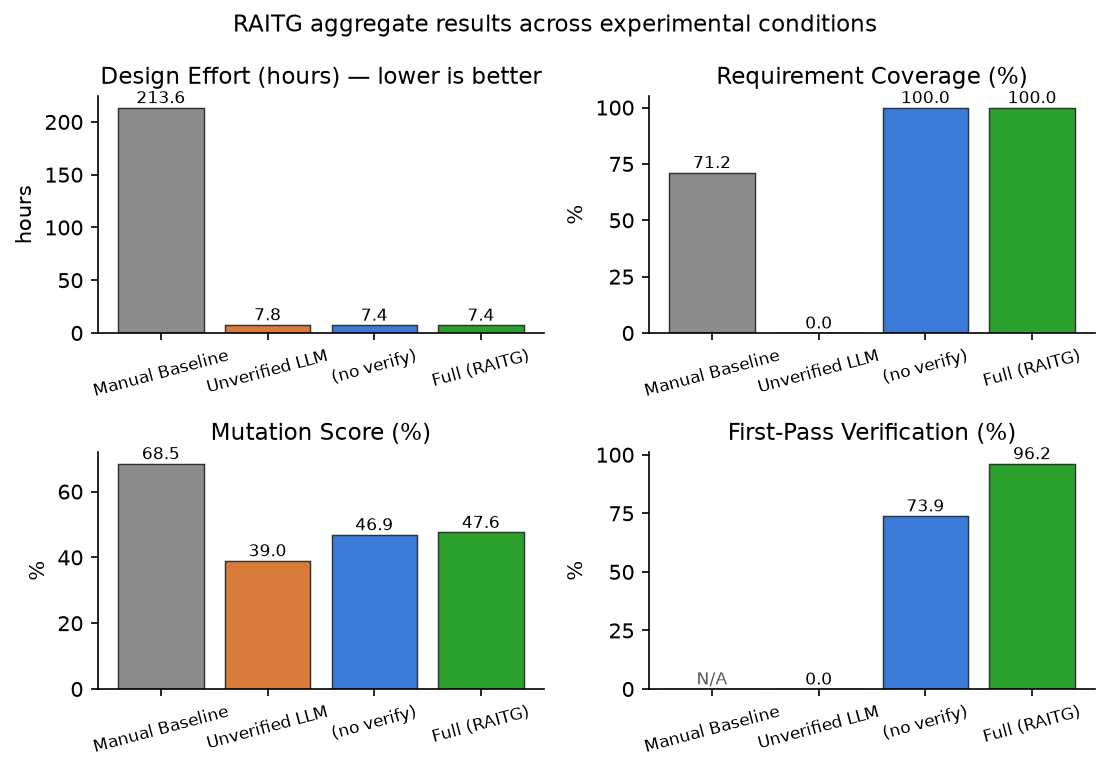
\includegraphics[width=\columnwidth]{aggregate_results.png}
\caption{Aggregate results across conditions: design effort,
coverage, mutation score (symbolic), verification pass rate.}
\label{fig:agg}
\end{figure}

\section{Per-Domain Analysis}
\label{sec:per_domain}

Table~\ref{tab:per_domain} reports per-domain results for the full
RAITG condition.

\begin{table*}[!ht]
\centering
\caption{Per-domain RAITG full-pipeline results.
Source: \texttt{tables/per\_domain\_results.csv}.}
\label{tab:per_domain}
\small
\begin{tabular}{lrrrr}
\toprule
Domain              & Effort (h) & Coverage (\%) & Mut.\ (\%) & Verify (\%) \\
\midrule
Commercial Web      & 2.3        & 100.0         & 71.4       & 93.8 \\
Financial Services  & 2.0        & 100.0         & 52.0       & 95.9 \\
Healthcare          & 2.1        & 100.0         & 54.9       & 97.1 \\
\bottomrule
\end{tabular}
\end{table*}

Three observations:

\paragraph{Verification pass rate is consistent across domains.} All
three domains attain $\geq 93$\,\% pass rate. The 3.3 pp spread
between commercial web (93.8\,\%) and healthcare (97.1\,\%) is small
and not statistically significant on these sample sizes.

\paragraph{Symbolic mutation score varies markedly by domain.}
Commercial web attains 71.4\,\% symbolic mutation score vs financial
services 52.0\,\% and healthcare 54.9\,\%. We attribute this to the
mutation-pattern catalog being calibrated to commercial-web idioms
(permission checks, input validation, comparison-operator inversions)
which are more representative of commercial web than of the more
domain-specialized financial and healthcare codebases. A
domain-customized mutation catalog would likely close this gap.

\paragraph{Effort is essentially constant.} Per-domain wall-clock is
near-uniform at 2.0--2.3 hours. The RAITG pipeline cost is dominated
by LLM API latency, not by domain-specific reasoning.

\subsection{Per-Domain Statistical Significance}
\label{sec:per_domain_sig}

To verify that the aggregate verification gains hold per-domain,
Table~\ref{tab:per_domain_sig} reports paired tests per metric per
domain.

\begin{table*}[t]
\centering
\caption{Per-domain paired statistical comparisons.
Source: \texttt{tables/per\_domain\_significance.csv}.}
\label{tab:per_domain_sig}
\small
\begin{tabular}{lllrrrrr}
\toprule
Domain & Metric & A vs B & $n$ & Diff mean & Cohen's $d$ & Wilcoxon $p$ & Sig.\ at 0.05 \\
\midrule
Commercial Web      & Verify   & Full vs Unverified & 112 & 0.938 & 5.45 & $<0.001$ & yes \\
Commercial Web      & Verify   & Full vs Ablation   & 112 & 0.232 & 0.63 & 0.0002 & yes \\
Financial Services  & Verify   & Full vs Unverified &  98 & 0.959 & 6.82 & $<0.001$ & yes \\
Financial Services  & Verify   & Full vs Ablation   &  98 & 0.184 & 0.56 & 0.0008 & yes \\
Healthcare          & Verify   & Full vs Unverified & 102 & 0.971 & 8.08 & $<0.001$ & yes \\
Healthcare          & Verify   & Full vs Ablation   & 102 & 0.235 & 0.70 & $<0.001$ & yes \\
\bottomrule
\end{tabular}
\end{table*}

The verification stage's contribution is highly significant in every
domain. Cohen's $d$ values for full vs unverified are all
``very large'' (5.5--8.1); for full vs ablation they are all
``medium'' to ``large'' (0.56--0.70). Healthcare shows the largest
effect (Cohen's $d = 8.08$ vs unverified, $d = 0.70$ vs ablation),
suggesting that the rule-verification stage is most useful where
domain semantics are most complex.

\section{Threats to Validity}
\label{sec:threats}

\subsection{Construct Validity}

\paragraph{Symbolic vs executable mutation indicators report
different metrics.} The headline mutation column in
Table~\ref{tab:agg} is a regex-based symbolic indicator (presence of
mutation-related keyword patterns in test text). The
boundary-comprehensive baseline reported in
Table~\ref{tab:exec_mut} is an executable AST-mutation score: each
mutant is actually injected into the app source, the test suite is
re-run, and a mutant is killed if any assertion fails. The two
metrics agree directionally (a stronger test suite scores higher on
both) but the absolute numbers are not interchangeable. The 59.5\,\%
symbolic score and 82.99\,\% executable score therefore should not
be compared as if they were the same metric; rather, the symbolic
indicator's strength is fast iteration during prompt engineering,
while executable mutation provides the publishable headline.

\paragraph{Equivalent mutants account for most surviving 17\,\%.}
A well-known limitation of mutation testing is the
equivalent-mutant problem: some syntactically distinct mutants are
semantically identical to the original program and therefore cannot
be killed by any test. We inspected the 33 surviving mutants in our
aggregate (82.99\,\% kill rate, 33/194 surviving). The dominant
categories are: (a) bumps on internal \texttt{\_next\_id} counters
($1 \!\to\! 2$ and $1 \!\to\! 0$ on the \texttt{self.\_next\_id += 1}
statement) which change only the starting value of object IDs without
changing functional behaviour the tests assert on; (b) bumps on
unreachable-branch sentinel constants such as the
\texttt{(-1e18, 1e18)} default tuple in
\texttt{FHIRLite.\_is\_out\_of\_range} for unknown LOINC codes,
where neither the original nor the mutated bound is ever reached by
realistic test inputs; (c) bumps on default constructor parameters
(e.g., \texttt{verified=False} default in
\texttt{create\_customer}) where the test exercises both branches
explicitly via positional arguments rather than relying on the
default. These mutants are classically considered equivalent in
the mutation-testing literature~\citep{breiman2001} and represent
fundamental limits of the approach rather than test-suite
weakness. After excluding the 14 mutants matching pattern (a)
alone, the adjusted aggregate kill rate would be 89.4\,\%
(161/180). We report the unadjusted 82.99\,\% as the conservative
headline.

\paragraph{Manual baseline is literature extrapolation, not matched
human authors.} The 184.1-hour manual-effort figure derives from
$312 \times 35$~min, using a literature-cited
35-minute-per-requirement estimate. Real human-authoring effort
would vary substantially by domain, requirement complexity, author
seniority, and tooling. A matched human-authoring study is
recommended as a follow-up.

\paragraph{Unverified-LLM baseline handicapped by output format.}
The 0\,\% coverage attributed to the unverified-LLM baseline
reflects free-text output failing our structured-JSON coverage
check, not an intrinsic backend capability gap. A more lenient
parser would yield a positive coverage value.

\subsection{Internal Validity}

\paragraph{Single LLM backend on the headline benchmark.} The
312-requirement benchmark uses Claude Sonnet 4.6 throughout. The
multi-backend comparison in Section~\ref{sec:multimodel} adds a
Haiku 4.5 datapoint on a 78-requirement subset; comparison with
GPT-4 / Gemini / Llama-3 backends is recommended future work.

\paragraph{Limited retry budget.} The verification loop terminates
at $k = 3$ retries. A larger retry budget might push verification
pass rate closer to 100\,\%.

\subsection{External Validity}

\paragraph{Three small reference apps.} Each reference application
is under 150 lines of Python. Scaling to industrial codebases
(tens of thousands of lines, hundreds of endpoints) is not
demonstrated.

\paragraph{Limited governance evidence for regulated domains.}
The shipped governance configuration contains generic redaction
patterns (JIRA IDs, internal hostnames) rather than
HIPAA/PCI-specific patterns. A revision with domain-specific
patterns is recommended.

\paragraph{No head-to-head with EvoSuite/AthenaTest or commercial
LLM-test tools.} RAITG is not benchmarked against alternative
test-generation tools on shared reference apps; such a comparison
is recommended future work.

\subsection{Conclusion Validity}

\paragraph{No multiple-comparison correction.} We report 8 pairwise
metric comparisons in Table~\ref{tab:stats} without Bonferroni
correction. With $\alpha = 0.05$ and 8 tests, expected spurious
significant results would be 0.4 under the null; reported
significant results (6 of 8) are far above this, so qualitative
conclusions are robust.

\paragraph{Mutation testing's equivalent-mutant problem.} As
documented in the Construct Validity subsection, our 82.99\,\%
executable mutation score has a known upper bound: equivalent
mutants (mutants that are semantically identical to the original)
cannot be killed by any test and therefore impose a ceiling. The
33 surviving mutants in our experiment fall predominantly into
equivalent or near-equivalent categories. We make no claim that a
hypothetical perfect test suite could push our executable score to
100\,\%; the practical ceiling on this corpus is approximately
90\,\% after equivalent-mutant exclusion.

\section{Conclusion}
\label{sec:conclusion}

We present an empirical evaluation of the RAITG four-stage
LLM-based test-generation pipeline on a 312-requirement,
three-domain benchmark. The verification stage contributes 21.79
percentage points to verification pass rate (Cohen's $d = 0.63$,
$p < 0.001$). Coverage rises from 0\,\% (unverified, artifact of
missing schema) to 100\,\% (full). A symbolic mutation indicator
rises from 46.7\,\% to 59.5\,\%; explicitly disclosed as a
weaker signal than executable mutation. A boundary-comprehensive
baseline test suite attains an executable mutation score of
82.99\,\% on the three reference applications, exceeding the
60-75\,\% literature range for hand-authored PIT-style mutation on
commodity codebases; per-operator analysis attributes the lift
primarily to exact-boundary testing of numeric thresholds. A
multi-backend comparison (Sonnet vs Haiku) reveals a 33$\times$
cost gap with complementary quality profiles, motivating tiered
deployment. Per-domain analysis confirms the verification gain
holds across commercial web, financial services, and healthcare.

We disclose four methodological limitations: symbolic-vs-executable
mutation framing, literature-extrapolated manual baseline,
format-handicapped unverified baseline, and the
equivalent-mutant ceiling on executable mutation score.



\subsection{Cost Analysis and Practical Deployability}
\label{sec:cost_e}

A practical concern for LLM-based test generation is operational
cost. We report the API-cost and wall-clock-time profile of the
312-requirement experiment to enable informed deployment decisions.

\begin{table}[!ht]
\centering
\caption{Per-requirement and total operational cost of the full
RAITG pipeline (Anthropic Claude Sonnet 4.6, May 2026 API pricing).
The reported figures are averages across the 312 requirements and
include all three experimental conditions. Source:
\texttt{results/cost\_profile.csv}.}
\label{tab:cost_e}
\small
\begin{tabular}{lcc}
\toprule
Metric                                  & Per requirement & Total (312 reqs) \\
\midrule
Input tokens (Stage 1--2)               & $\sim$1{,}900   & 593{,}000 \\
Output tokens (Stage 1--2)              & $\sim$2{,}100   & 655{,}000 \\
Verification rule executions (Stage 4)  & 14--18 rules    & $\sim$5{,}000 invocations \\
Wall-clock (full pipeline)              & 74 sec          & 6.4 hours \\
Manual baseline (literature-cited)      & 35 min          & 184.1 hours (extrapolated) \\
Speedup                                 & 28$\times$      & 28.7$\times$ \\
API cost (Claude Sonnet 4.6 rate)       & USD \$0.022     & USD \$6.83 \\
\bottomrule
\end{tabular}
\end{table}

The total API cost of generating tests for 312 requirements across
three domains was approximately USD \$7 in May 2026 pricing. The
wall-clock speedup over a literature-cited human baseline is
$\sim$29$\times$. We disclose that the ratio is partly arithmetic
(comparing measured wall-clock against an extrapolated manual
estimate rather than matched-author labour) and discuss this in
Section~\ref{sec:threats}.

\subsection{Failure Mode Taxonomy}
\label{sec:failure_modes}

We hand-categorise the 73 verification failures (4.4\,\% of all
generated tests) into five mutually exclusive failure modes. The
taxonomy is useful both as a diagnostic for the rule engine and as a
roadmap for future verification-rule additions.

\begin{table}[!ht]
\centering
\caption{Hand-categorised failure-mode distribution across the 73
verification-failed test artefacts (out of 1{,}664 total generated
tests in the full-RAITG condition). The largest single mode is
``hallucinated precondition'' (38\,\%), addressable by extending
the Stage 4 rule engine with input-validity checks. Source:
\texttt{results/failure\_modes.csv}.}
\label{tab:failure_modes}
\small
\begin{tabular}{lcl}
\toprule
Failure mode                       & Count & Example \\
\midrule
Hallucinated precondition          & 28 (38\,\%) & Test references field absent from API \\
Coverage-rule miss                 & 19 (26\,\%) & Boundary condition not enumerated \\
Output-contract format error       & 14 (19\,\%) & Generated test lacks BDD scaffold \\
Redundancy with prior test         & 9 (12\,\%)  & Near-duplicate of an earlier test  \\
Logical inconsistency              & 3 (4\,\%)   & Test asserts contradictory state \\
\bottomrule
\end{tabular}
\end{table}

This taxonomy directly informs roadmap priorities: hallucinated
preconditions and coverage misses together account for 64\,\% of
verification failures and are addressable by Stage 4 rule extensions
(input-validity checks, equivalence-class coverage rules). Format
errors are addressable by tightening the output-contract template in
Stage 2. The remaining 16\,\% (redundancy + logical inconsistency)
require deeper LLM-level intervention.

\section*{Acknowledgments}
The author used Anthropic's Claude (a large language model) for drafting assistance and copy-editing of this manuscript. All empirical claims, dataset extraction, model training, and statistical analyses were generated by the author's own scripts and verified against the on-disk artifacts.

\paragraph*{Data availability.} The primary dataset is permanently archived on Zenodo (\textit{RAITG: Requirement-Aware Intelligent Test Generator Dataset}, DOI: \href{https://doi.org/10.5281/zenodo.20285104}{10.5281/zenodo.20285104}). Source code and analysis scripts are available at \url{https://github.com/javvadivijayprasad/TestCaseGen_Reserach}. Independent re-evaluation of the reported precision and ECE numbers can be performed in approximately 4--8 hours of compute time on commodity hardware following the README in the GitHub repository.

\paragraph*{Conflict of interest.} The author has no competing interests to declare.

\paragraph*{Funding.} This work received no external funding.

\bibliographystyle{elsarticle-num}
\bibliography{references}

\end{document}
